\chapter{Implementation of Typing Test Scenario and Metrics}

\section{Introduction}
This chapter details the implementation of a comprehensive typing test scenario designed to evaluate user performance with different virtual keyboard types in a virtual reality (VR) environment. The scenario includes various elements such as user input handling, data collection, phrase management, error tracking, and database integration to provide a robust framework for testing and analysis.

\section{Typing Test Scenario}

\subsection{Overview of the Typing Test Scenario}
The typing test scenario aims to assess the typing performance of users using different keyboard configurations in a VR environment. Specifically, the test compares the MRTK (Mixed Reality Toolkit) Keyboard with a custom virtual keyboard designed for this study. The MRTK Keyboard, part of Microsoft's Mixed Reality Toolkit, provides a standardized virtual input method that includes features such as spatial awareness, robust input handling, and support for hand and eye tracking \cite{mrtk_keyboard}. It is designed to facilitate ease of use and seamless interaction within virtual reality environments, making it an ideal choice for evaluating virtual text entry.
\begin{figure}[h]
    \centering
    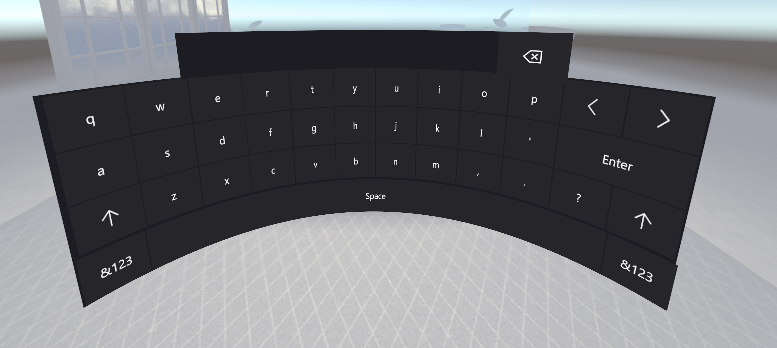
\includegraphics[width=0.8\textwidth]{Scenario/MRTK_KEyboard.PNG} % Replace with your image file name
    \caption{ \centering MRTK Keyboard interface showing a curved QWERTY layout designed for virtual reality environments inisde unity.}
    \label{fig:mrtk_keyboard}
\end{figure}\\ \\
The custom virtual keyboard, on the other hand, was created using Blender \ref{sec:Virtual Keyboard Conception} to incorporate enhanced haptic feedback mechanisms and ergonomic design tailored to improve user interaction and typing efficiency. This custom keyboard aims to address the limitations of existing virtual keyboards by providing a more intuitive and immersive typing experience through advanced haptic feedback and ergonomic considerations. 
\begin{figure}[h]
    \centering
    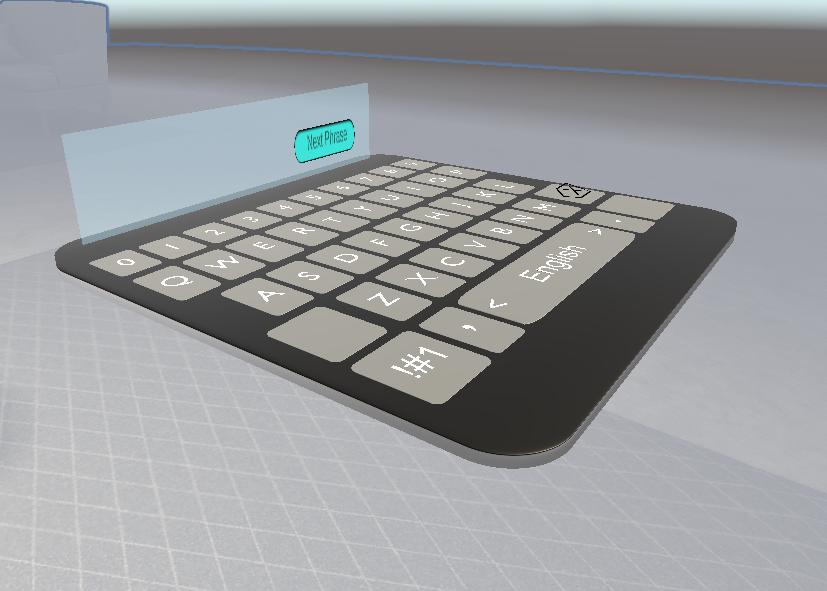
\includegraphics[width=0.8\textwidth]{Scenario/Custom_keyboard.PNG} % Replace with your image file name
    \caption{ \centering Custom virtual keyboard interface designed with enhanced haptic feedback and ergonomic features for improved typing efficiency in VR inside unity.}
    \label{fig:mrtk_keyboard}
\end{figure}\\ \\
The system captures detailed user input data, records performance metrics, and manages the flow of the test to ensure a comprehensive evaluation. The phrases used in the test are sourced from Scott MacKenzie's phrase sets, which are widely recognized in the field of text entry research. MacKenzie's phrase sets are designed to provide a standardized basis for evaluating text entry methods, featuring a wide range of commonly used words and phrases that reflect typical typing scenarios. These phrase sets are carefully curated to balance frequency and representativeness, ensuring that the typing tasks are both realistic and challenging \cite{mackenzie_phrase_set}. \\ \\
By using these standardized phrases, the study can reliably measure typing performance metrics such as Words Per Minute (WPM) and Error Rate (ER), providing valuable insights into the efficiency and accuracy of each keyboard configuration. The consistent use of MacKenzie's phrase sets allows for comparability with other studies in the field, facilitating a broader understanding of virtual text entry performance. 
\subsection{User Input Handling}
The system continuously monitors the user's typing input in a designated text field, tracking each keystroke and identifying any mistakes made during the typing process. This allows for real-time data collection and analysis of user performance.

\subsection{Data Collection}
Detailed data about the typing session is collected, including the time taken, the number of keystrokes, and the accuracy of the typed text compared to the expected text. After the user finishes typing a phrase, the system records this data and saves it inside a third-party database.

\subsection{Phrase Management}
The test involves typing a series of phrases. The system loads a new phrase for the user to type and displays it on the screen. Once the user finishes typing a phrase, the system prepares the next phrase, ensuring a continuous flow of the test.

\subsection{Error and Accuracy Tracking}
The system not only counts the total keystrokes but also keeps track of incorrect keystrokes, helping to measure the user's typing accuracy. It calculates various metrics such as error rate, accuracy in characters, accuracy in words, and typing speed.

\subsection{Interactive Elements}
Interactive elements such as a button allow the user to proceed to the next phrase. This ensures that users have control over the transition between different phrases and keyboard types.

\subsection{Data Storage}
All the typing data collected during the test is stored in a database. This data includes details like the typed text, the expected text, the time taken, and various accuracy metrics. Storing this data allows for detailed post-test analysis.

\subsection{Configuration and Setup}
Before starting the test, the system loads configuration settings such as the types of keyboards to be tested and other parameters that guide the test process. The configuration settings include:
\begin{itemize}
    \item Names of the keyboards to be tested.
    \item Number of phrases the user should type in both the training scene and the testing scene.
    \item Waiting duration between different keyboards of the test.
    \item Vibration and force feedback settings for the gloves.
\end{itemize}

\subsection{Scene Management}
The test scenario involves three main scenes: Training, Testing, and Waiting.
\begin{itemize}
    \item \textbf{Training Scene:} The user practices typing to get familiar with the keyboard.
    \item \textbf{Testing Scene:} The user is tested on their typing performance.
    \item \textbf{Waiting Scene:} The user waits while the system transitions between different keyboard types.
\end{itemize}

\subsection{Scene Occurrences}
For each keyboard, the sequence of scenes is:
\begin{enumerate}
    \item Training Scene
    \item Testing Scene
    \item Waiting Scene
\end{enumerate}

If we have 2 keyboards to test, the sequence repeats for each keyboard. Therefore, for 2 keyboards, the scenes will appear as follows:
\begin{itemize}
    \item Training Scene: 1 time per keyboard $\times$ 2 keyboards = 2 times
    \item Testing Scene: 1 time per keyboard $\times$ 2 keyboards = 2 times
    \item Waiting Scene: 1 time per 2 keyboards
\end{itemize}

\subsection{Adjustable Settings in the Database}
\begin{itemize}
    \item \textbf{Vibration and Force Feedback:} The vibration and force feedback settings of the gloves used in the test can be adjusted via the database. This ensures that the feedback experienced by the user is tailored to the specific requirements of the test scenario.
    \item \textbf{Waiting Duration:} The duration in seconds of the waiting period between different types of keyboards of the test can be adjusted in the database.
    \item \textbf{Keyboard Names:} The names and types of keyboards to be tested can be updated in the database, making the system adaptable to different testing needs.
    \item \textbf{Number of Phrases:} The number of phrases that the user is required to type in both the training and testing scenes can be configured in the database, ensuring the test is appropriately challenging and comprehensive.
\end{itemize}

\subsection{Detection of a Finished Phrase}
The system detects that a phrase is finished when the user types the expected number of words of the expected phrase to type and the phrase ends with a period. Upon detection, the system:
\begin{itemize}
    \item Records the typing data for the completed phrase.
    \item Makes the button for proceeding to the next phrase interactable.
\end{itemize}

\section{Workflow Summary}
The workflow of the typing test scenario involves the following steps:
\begin{enumerate}
    \item \textbf{Initialization:} The system sets up the test environment and prepares the first phrase.
    \item \textbf{Typing Phase:} The user types the displayed phrase, and the system tracks keystrokes and errors in real-time.
    \item \textbf{Detection of Completion:} The system detects when the user has finished typing the phrase by checking word count and punctuation.
    \item \textbf{Data Recording:} Upon completion of each phrase, the system records the typing data.
    \item \textbf{Phrase Transition:} The user moves to the next phrase by clicking a button.
    \item \textbf{Scene Transition:} The system transitions between Training, Testing, and Waiting scenes as needed for each keyboard type.
\end{enumerate}

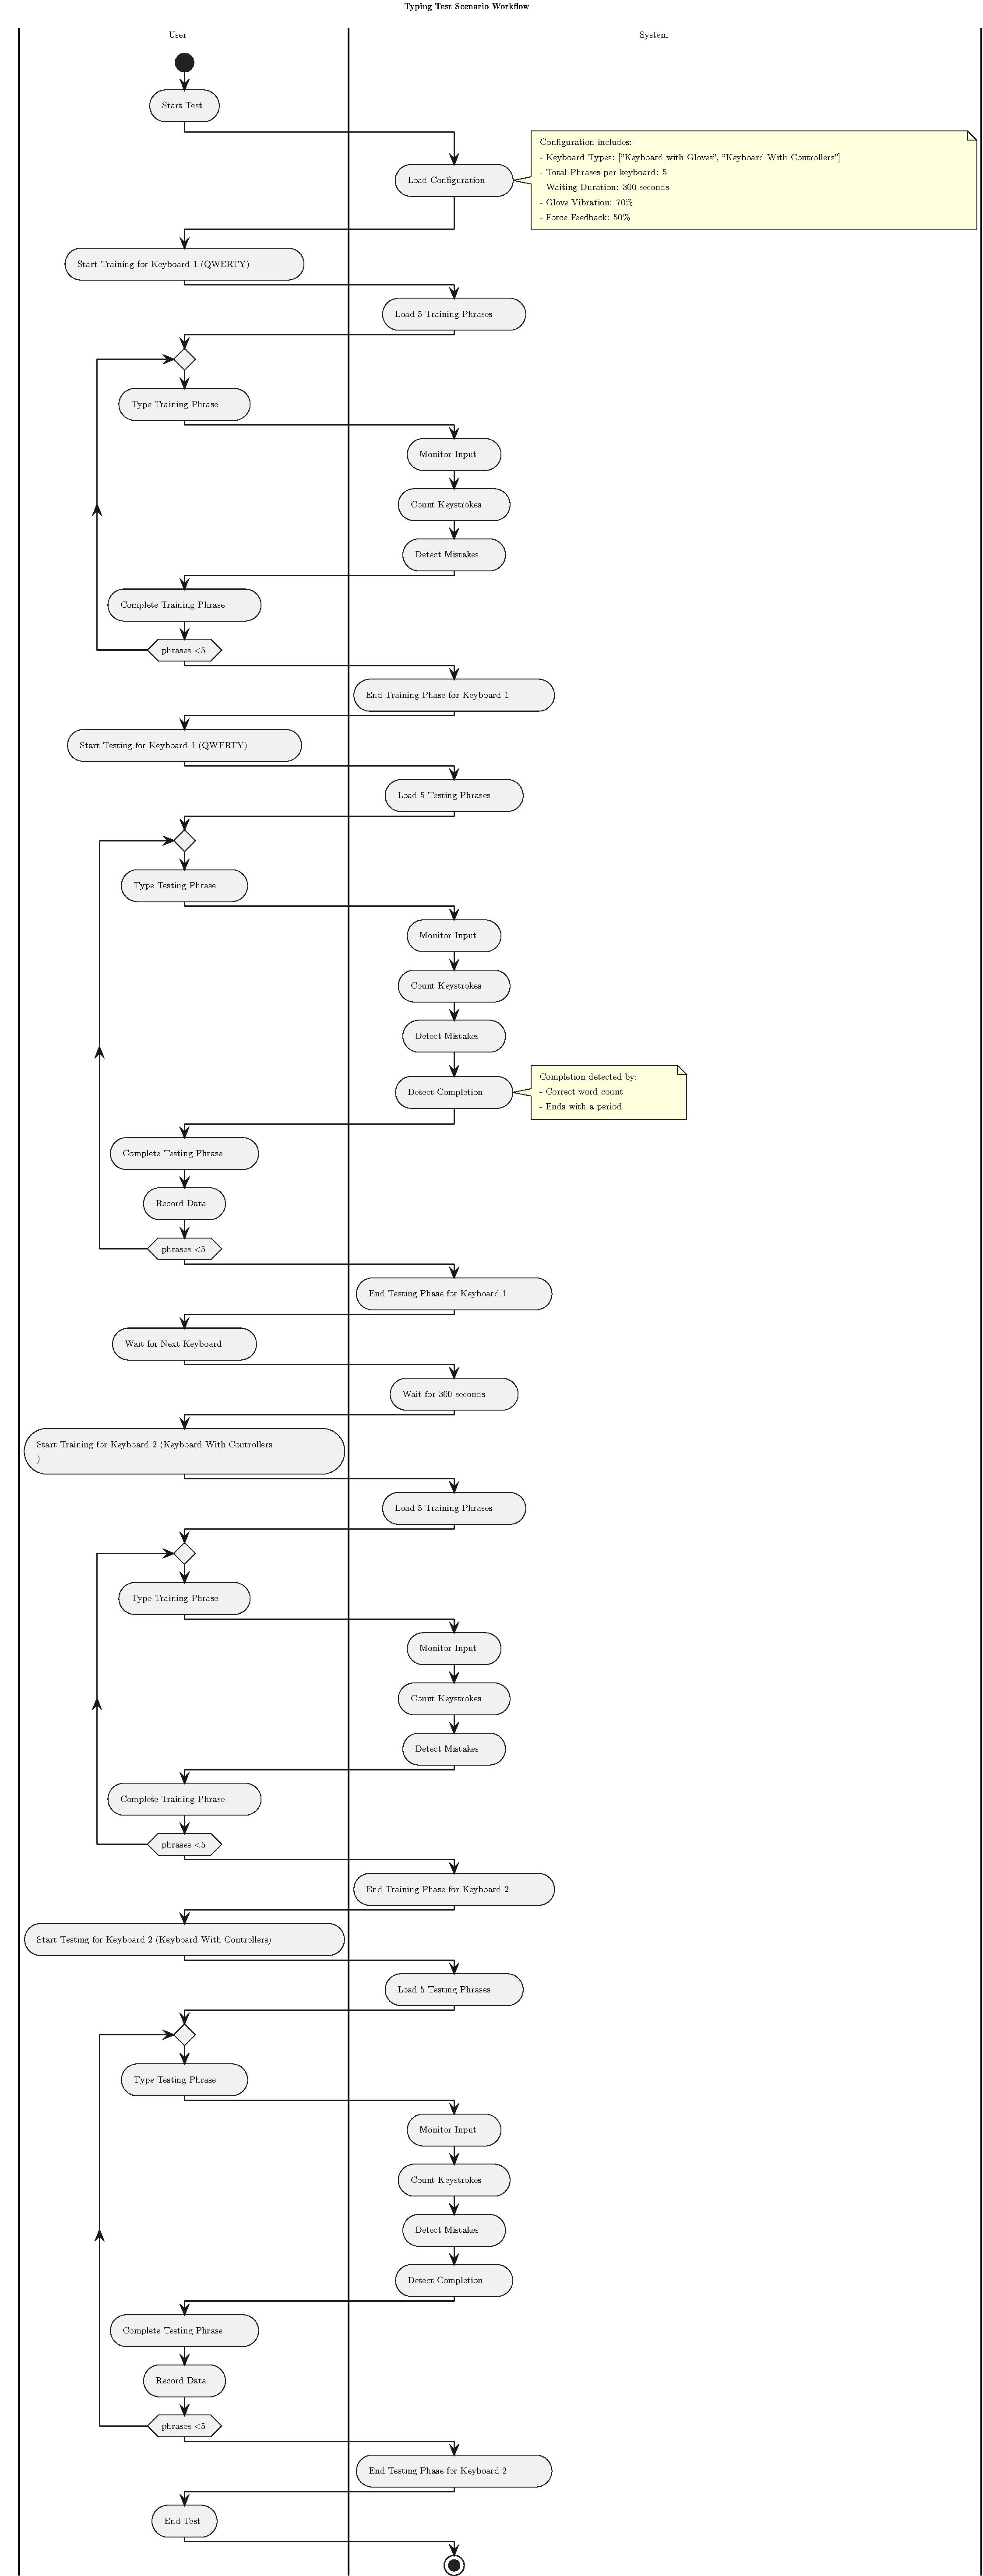
\includepdf[pages=-, landscape=true, fitpaper=true]{Scenario/scenario_PDF2.pdf}

\section{Typing Performance Metrics and Database Registration}

\subsection{Metrics Overview}
The performance of users is analyzed using several metrics. These metrics provide a comprehensive understanding of the user's typing efficiency and accuracy in the VR environment.

\begin{itemize}
    \item \textbf{Error Rate:} This metric calculates the percentage of errors by computing the Levenshtein distance between the expected text and the typed text. The Levenshtein distance \(d(s, t)\) is a measure of the minimum number of single-character edits (insertions, deletions, or substitutions) required to change one word into the other. The formula used to calculate the error rate is:
    \begin{equation}
    \text{Error Rate} = \frac{d(s, t)}{\max(\text{Length of Expected Text}, \text{Length of Typed Text})} \times 100
    \end{equation}
    where \(d(s, t)\) is the Levenshtein distance between the strings \(s\) (expected text) and \(t\) (typed text).

    \item \textbf{Character-Level Accuracy:} This metric measures the accuracy at the character level by calculating the Levenshtein distance and then determining the percentage of characters typed correctly. The formula used is:
    \begin{equation}
    \text{Accuracy in Characters} = 100 - \left( \frac{d(s, t)}{\text{Length of Expected Text}} \times 100 \right)
    \end{equation}
    This metric highlights the proportion of correctly typed characters relative to the expected characters.

    \item \textbf{Word-Level Accuracy:} This metric assesses the accuracy at the word level. It compares each word in the expected text with the corresponding word in the typed text, counting the mismatches. The formula used is:
    \begin{equation}
    \text{Accuracy in Words} = 100 - \left( \frac{\text{Number of Words with Errors}}{\text{Number of Words in Expected Text}} \times 100 \right)
    \end{equation}
    This metric provides insight into how accurately the user can reproduce words as opposed to individual characters.

    \item \textbf{Keystroke-Level Accuracy:} This metric evaluates the accuracy based on the number of incorrect keystrokes out of the total keystrokes made. The formula used is:
    \begin{equation}
    \text{Accuracy in Keystrokes} = 100 - \left( \frac{\text{Incorrect Keystrokes}}{\text{Total Keystrokes}} \times 100 \right)
    \end{equation}
    This metric helps in understanding the precision of each keystroke made by the user.

    \item \textbf{Typing Speed:} This metric calculates typing speed in words per minute (WPM). It assumes that an average word consists of five characters. The formula used is:
    \begin{equation}
    \text{Typing Speed} = \left( \frac{\text{Number of Characters Typed}}{5} \right) \div \left( \frac{\text{Time Taken in Seconds}}{60} \right)
    \end{equation}
    Typing speed is an important metric to gauge how quickly a user can type, which is crucial for evaluating productivity.

    \item \textbf{Keystrokes per Character:} This metric calculates the number of keystrokes per character typed. The formula used is:
    \begin{equation}
    \text{Keystrokes per Character} = \frac{\text{Keystroke Count}}{\max(1, \text{Character Count})}
    \end{equation}
    This metric indicates the efficiency of the user's typing, with a lower value signifying higher efficiency.

    \item \textbf{Levenshtein Distance:} The Levenshtein distance \(d(s, t)\) between two strings \(s\) and \(t\) is defined as the minimum number of single-character edits (insertions, deletions, or substitutions) required to transform \(s\) into \(t\). The distance can be computed using a dynamic programming approach where \(d(i, j)\) represents the distance between the first \(i\) characters of \(s\) and the first \(j\) characters of \(t\). The recursive formula is:
    \begin{equation}
    d(i, j) = \begin{cases} 
      i & \text{if } j = 0 \\
      j & \text{if } i = 0 \\
      \min \begin{cases} 
      d(i-1, j) + 1 \\ 
      d(i, j-1) + 1 \\ 
      d(i-1, j-1) + (1 - \text{match}(s_i, t_j))
      \end{cases} & \text{otherwise}
   \end{cases}
    \end{equation}
    Here, \(\text{match}(s_i, t_j)\) is 1 if the characters \(s_i\) and \(t_j\) are the same, and 0 otherwise. This metric provides a foundational measure of typing accuracy by quantifying how similar the typed text is to the expected text.
\end{itemize}

\subsection{Database Registration and Storage}
The application establishes a connection to the MongoDB database. This connection is initiated during the startup process, ensuring that the database connection is established when the application begins running. The necessary collections for storing user data and configuration settings are initialized at this point.

\subsubsection{Inserting Typing Data}
Typing performance data, encapsulated in a structured format, is inserted into the MongoDB collection. This data includes various metrics such as:
\begin{itemize}
    \item \textbf{Expected text:} The predefined text that the user is expected to type during the test.
    \item \textbf{Typed text:} The actual text that the user types, which is recorded for analysis.
    \item \textbf{Time taken to type:} The total time (in seconds) that the user takes to complete typing the expected text.
    \item \textbf{Keystroke count:} The total number of keystrokes made by the user during the typing session.
    \item \textbf{Error rate:} The percentage of errors made by the user, calculated using the Levenshtein distance between the expected text and the typed text.
    \item \textbf{Character-level accuracy:} The accuracy of the typed text at the character level, indicating how many characters were typed correctly relative to the expected text.
    \item \textbf{Word-level accuracy:} The accuracy of the typed text at the word level, indicating how many words were typed correctly relative to the expected text.
    \item \textbf{Keystroke-level accuracy:} The accuracy based on the number of incorrect keystrokes out of the total keystrokes made.
    \item \textbf{Typing speed:} The typing speed measured in words per minute (WPM), assuming an average word consists of five characters.
    \item \textbf{Keystrokes per character:} The number of keystrokes made per character typed, indicating the efficiency of the user's typing.
    \item \textbf{Session time:} The total duration of the typing session, from start to finish.
    \item \textbf{User ID:} A unique identifier for the user, used to track individual performance data.
    \item \textbf{Keyboard type:} The type of keyboard used by the user during the typing session, which could influence performance.
\end{itemize}

To illustrate the data collected during the typing test, we include two examples of documents stored in MongoDB. The first example shows a case where the phrase is typed correctly, and the second example shows a case where the phrase contains errors.

\begin{figure}[h]
    \centering
    \begin{subfigure}[b]{0.45\textwidth}
        \centering
        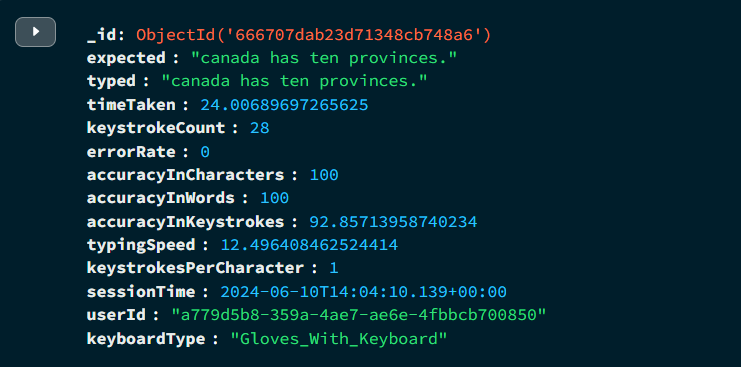
\includegraphics[width=\textwidth]{Scenario/Correct_Phrase.PNG}
        \caption{Correctly typed phrase}
        \label{fig:correct_case}
    \end{subfigure}
    \hfill
    \begin{subfigure}[b]{0.45\textwidth}
        \centering
        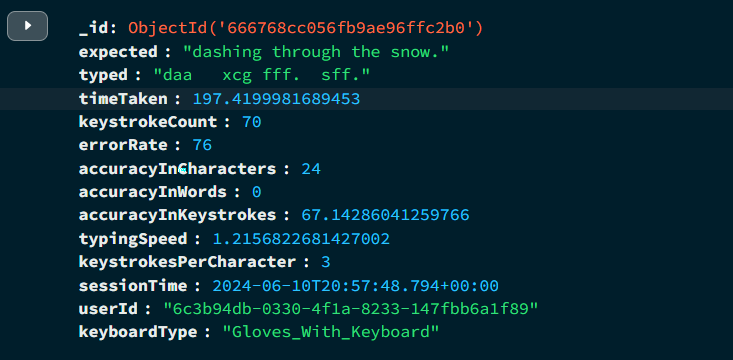
\includegraphics[width=\textwidth]{Scenario/wrong_Phrase.PNG}
        \caption{Incorrectly typed phrase}
        \label{fig:incorrect_case}
    \end{subfigure}
    \caption{Examples of typing data stored in MongoDB}
    \label{fig:database_examples}
\end{figure}

\subsubsection{Fetching Global Configuration}
Global configuration settings are retrieved from the database. The application queries the configuration collection and extracts various settings related to gloves configuration, keyboards to test, session settings, and waiting duration. These configurations are then used to adjust the application’s behavior based on the retrieved settings.

\subsubsection{Inserting User Data}
User data, encapsulated in a structured format, is inserted into the MongoDB collection. This data includes:
\begin{itemize}
    \item User ID
    \item User name
    \item User age
    \item User sex
\end{itemize}

